\chapter{Funktioner}
För ala reella tall $a\neq 0$ gäller att $a\cdot \frac{1}{a}=1$.
Talet $1/a$ kallas för den \emph{multiplikativa inversen} till $a$.
Den multiplikativa inversen definieras med hjälp av det speciellt talet 1 (ettan) som har den \emph{unika} egenskapen att $a\cdot 1 = 1\cdot a=a$ $\forall a\in \mathbb{R}$.
Om vi istället för de reella talen nu tänker oss funktioner och istället för multiplikation tänker oss komposition, alltså $f\circ g$, finns det då en "etta"?
Ja! Funktionen $e(x)=x$ blir en etta eftersom $f\circ e(x)=f(e(x))=f(x)$ och $e\circ f(x)=e(f(x))=f(x)$ så alltså gäller att $f\circ e=e\circ f=f$ för alla funktioner $f$.
Med $e(x)=x$ som "etta" är det naturligt att fråga sig; givet en funktion $f$, finns det då en annan funktion $g$ så att $f\circ g=g\circ f=e$?
Ja! Funktionen $g(x)=\frac{1}{f(x)}$ blir en sådan funktion eftersom $f\circ g(x)=f(\frac{1}{f(x)})=\frac{1}{f(x)}$ och $g\circ f(x)=\frac{1}{f(f(x))}=\frac{1}{f(x)}$ så alltså gäller att $f\circ g=g\circ f=e$.
Detta gäller dock endast om $f$ är injektiv, alltså om $x_1\neq x_2\Rightarrow f(x_1)\neq f(x_2)$.
Funktionen $g$ kallas då för \emph{inversen} till $f$ och skrivs $f^{-1}$.
Geometriskt så representeras $f^{-1}$ som en spegelbild av $f$ i linjen $y=x$.
Lite grundläggande egenskaper för inverser:
\begin{itemize}
    \item $y=f^{-1}(x) \Leftrightarrow x=f(y)$
    \item $f\circ f^{-1}=f^{-1}\circ f=x$
    \item $(f^{-1})^{-1}(x)=f(x)$
\end{itemize}
Man kan också beräkna derivata av inversfunktionen som $\frac{d}{dx}(f^{-1}(x))=\frac{1}{f'(f^{-1}(x))}$
eftersom vi vet att $f(f^{-1}(x))=x\Rightarrow \frac{d}{dx}(f(f^{-1}(x)))=\frac{d}{dx}(x)=1$ och $\frac{d}{dx}(f(f^{-1}(x)))=$ \{kedjeregeln\} $=f'(f^{-1}(x))\cdot \frac{d}{dx}f^{-1}x\Rightarrow \frac{d}{dx}f^{-1}(x)=\frac{1}{f'(x^{-1}(x))}$.
\emph{Behöver inte bevisas på tentan.}
\section{Exponentialfunktioner}
En exponentialfunktion är en funktion på formen $f(x)=a^x$ där $a>0$.
Det gäller att $a^0=1$, $a^{x+y}=a^x\cdot a^y$, $a^{-x}=\frac{1}{a^x}$ och $(a^x)^y=a^{x\cdot y}$.
Vidare är funktionen $f(x)=a^x$ en \emph{injektiv} funktion, och därmed finns alltid en invers.
Denna invers kallas för \emph{$a$-logaritmen} och skrivs $f^{-1}(x)=\log_a(x)$.
För alla $a$-logaritmer gäller att
\begin{itemize}
    \item $y=\log_a(x) \Leftrightarrow x=a^y$
    \item $\log(1)=0$
    \item $\log_a(x\cdot y)=\log_a(x)+\log_a(y)$
    \item $\log_a(\frac{x}{y})=\log_a(x)-\log_a(y)$
    \item $\log_a(\frac{1}{x})=-\log_a(x)$
    \item $\log_a(x^y)=y\cdot \log_a(x)$
    \item $\log_a(x)=\frac{\log_b(x)}{\log_b(a)}$, om $a>0$ och $b>0$
\end{itemize}
Derivatan av $f(x)=a^x$ är $f'(x)=a^x\cdot \log_a(x)$.
Finns det ett tall $a$ så att $C=1$?
Ja, och det kallas $e\approx 2,718281828\ldots$.
Motsvarande $e$-logaritmen kallas för den \emph{naturliga logaritmen} och betecknas $\ln(x)$.
Genom detta fås att $\frac{d}{dx}a^x=\frac{d}{dx}e^{\ln(a^x)}=\frac{d}{dx}e^{x\cdot\ln(a)}=\ln(a)\cdot a^x$.
På motsvarande sätt gäller att $\frac{d}{dx}\ln(x)=\frac{1}{x}$, och $\frac{d}{dx}\log_a(x)=\frac{1}{x\cdot \ln(a)}$.
Exponentialfunktioner och logaritmer är oumbärliga för att modellera en mängd olika processer.
I synnerhet tillväxt-/avtagande-modellering.
\begin{figure}[h]
    \centering
    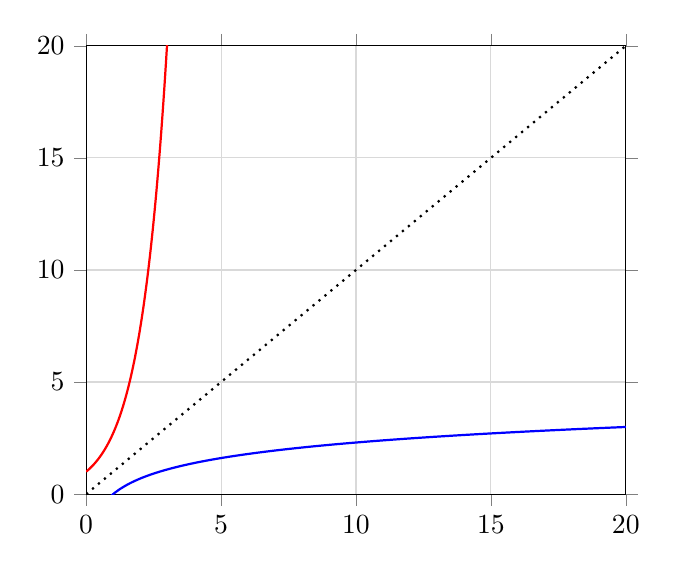
\begin{tikzpicture}
        \begin{axis}[
                xmin=0, xmax=20,
                xticklabel style={/pgf/number format/.cd,fixed},
                grid = major,
                grid style={gray!30},
                ymin=0,
                ymax= 20,
                axis background/.style={fill=white},
                tick align=outside
            ]
            \addplot[domain=0:3.5, red, thick, samples=200] {e^x};
            \addplot[domain=0.1:20, blue, thick, samples=200] {ln(x)};
            \addplot[domain=0:20, black, thick, dotted] {x};
        \end{axis}
    \end{tikzpicture}
    \caption{Kurvorna $y=e^x$ och $y=\ln(x)$}
\end{figure}
Jämfört med potensfunktionen $x^n$, $n>0$, så växer/avtar $e^x$ alltid snabbare och tvärtom för $\ln(x)$:
$\lim_{x\to \infty}\frac{x^n}{e^x}=0$, $\lim_{x\to -\infty}|x^n|e^x=0$, $\lim_{x\to\infty}\frac{\ln x}{x^n}=0$, $\lim_{x\to 0^+}x^n\cdot \ln x=0$.
Vad gäller för de primitiva funktionerna (indefinita integralerna) av $e^x$ och $\ln(x)$?
$\int e^x dx=e^x+C$, $\int \ln(x)dx=x\ln(x)-x+C$ (primitiv av $\ln(x)$ kan vi egentligen inte än).
För $\ln |x|$ gäller att $\frac{d}{dx}\ln |x|=\frac{1}{x}\cdot sgn(x)=\frac{1}{x}$, så $\int \frac{1}{x}dx=\ln |x|+C$.
Talet $e$ är intressant i sig, och omgärdas än idag av flera olösta matimatiska problem.
Det kan formuleras som följande kända gränsvärde: $e=\lim_{x\to\infty}(1+\frac{1}{n})^n$ och således gäller att $e^x=\lim_{x\to\infty}(1+\frac{x}{n})^n$.
\section{Inversa trigonometriska funktioner}
Funktionerna $\sin x$, $\cos x$ och $\tan x$ är periodiska och därmed inte injektiva på $\mathbb{R}$.
Av den anledningen saknas inversfunktioner.
Det går dock att begränsa dem så att de blir injektiva på ett kortare intervall.
$\arcsin x$, $\arccos x$ och $\arctan x$ har följande definitions- och värdemängder:
\begin{itemize}
    \item $\arcsin x$ $\mathcal{D}=[-1,1]$, $\mathcal{R}=[-\frac{\pi}{2},\frac{\pi}{2}]$
    \item $\arccos x$ $\mathcal{D}=[-1,1]$, $\mathcal{R}=[0,\pi]$
    \item $\arctan x$ $\mathcal{D}=[-\infty,\infty]$, $\mathcal{R}=[-\frac{\pi}{2},\frac{\pi}{2}]$
\end{itemize}
Man har följande derivator:
\begin{itemize}
    \item $\frac{d}{dx} \arcsin x=\frac{1}{\sqrt{1-x^2}}$
    \item $\frac{d}{dx} \arccos x=\frac{1}{\sqrt{1-x^e}}$
    \item $\frac{d}{dx} \arctan x=\frac{1}{1+x^2}$
\end{itemize}
\section{De hyperboliska funktionerna}
Släktingar till de trigonometriska funktionerna med många liknande egenskaper.
$\sinh x = \frac{e^x-e^{-x}}{2}$, $\cosh x = \frac{e^x+e^{-x}}{2}$
Precis som för $\sin$ och $\cos$, så är $\sinh$ en udda funktion och $\cosh$ en jämn funktion.
Den trigonometriska ettan gäller nästan (hyperboliska ettan!): $\cosh^2 x - \sinh^2 x = 1$.
För derivatorna gäller att $\frac{d}{dx}\sinh x = \cosh x$, $\frac{d}{dx}\cosh x = \sinh x$.
Man definierar $\tanh = \frac{\sinh}{\cosh}$och får att $\frac{d}{dx}$